% https://tex.stackexchange.com/a/13952/173708
\documentclass[border=15pt]{standalone}
\usepackage{tikz}
\usetikzlibrary{calc,patterns,decorations.pathmorphing,decorations.markings}

\begin{document}

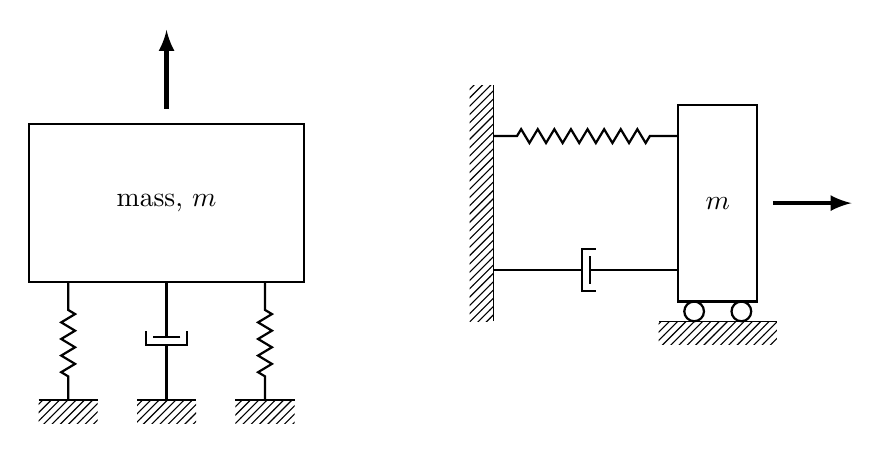
\begin{tikzpicture}[every node/.style={draw,outer sep=0pt,thick}]
  \tikzstyle{spring}=[thick,decorate,decoration={zigzag,pre length=0.3cm,post length=0.3cm,segment length=6}]
  \tikzstyle{damper}=[thick,decoration={markings,  
    mark connection node=dmp,
    mark=at position 0.5 with 
    {
      \node (dmp) [thick,inner sep=0pt,transform shape,rotate=-90,minimum width=15pt,minimum height=3pt,draw=none] {};
      \draw [thick] ($(dmp.north east)+(2pt,0)$) -- (dmp.south east) -- (dmp.south west) -- ($(dmp.north west)+(2pt,0)$);
      \draw [thick] ($(dmp.north)+(0,-5pt)$) -- ($(dmp.north)+(0,5pt)$);
    }
  }, decorate]

  \tikzstyle{ground}=[fill,pattern=north east lines,draw=none,minimum width=0.75cm,minimum height=0.3cm]

  \node (M) [minimum width=3.5cm,minimum height=2cm] {mass, $m$};

  \node (ground1) at (M.south) [ground,yshift=-1.5cm,xshift=-1.25cm,anchor=north] {};
  \draw (ground1.north west) -- (ground1.north east);
  \draw [spring] (ground1.north) -- ($(M.south east)!(ground1.north)!(M.south west)$);

  \node (ground2) at (M.south) [ground,yshift=-1.5cm,anchor=north] {};
  \draw (ground2.north west) -- (ground2.north east);
  \draw [damper] (ground2.north) -- ($(M.south east)!(ground2.north)!(M.south west)$);

  \node (ground3) at (M.south) [ground,yshift=-1.5cm,xshift=1.25cm,anchor=north] {};
  \draw (ground3.north west) -- (ground3.north east);
  \draw [spring] (ground3.north) -- ($(M.south east)!(ground3.north)!(M.south west)$);

  \draw [-latex,ultra thick] (M.north) ++(0,0.2cm) -- +(0,1cm);

  \begin{scope}[xshift=7cm]
    \node (M) [minimum width=1cm, minimum height=2.5cm] {$m$};

    \node (ground) [ground,anchor=north,yshift=-0.25cm,minimum width=1.5cm] at (M.south) {};
    \draw (ground.north east) -- (ground.north west);
    \draw [thick] (M.south west) ++ (0.2cm,-0.125cm) circle (0.125cm)  (M.south east) ++ (-0.2cm,-0.125cm) circle (0.125cm);

    \node (wall) [ground, rotate=-90, minimum width=3cm,yshift=-3cm] {};
    \draw (wall.north east) -- (wall.north west);

    \draw [spring] (wall.170) -- ($(M.north west)!(wall.170)!(M.south west)$);
    \draw [damper] (wall.10) -- ($(M.north west)!(wall.10)!(M.south west)$);

    \draw [-latex,ultra thick] (M.east) ++ (0.2cm,0) -- +(1cm,0);
  \end{scope}
\end{tikzpicture}

\end{document}